\documentclass[11pt,a4paper]{article}
\usepackage[utf8]{inputenc}
\usepackage[spanish]{babel}
\usepackage[T1]{fontenc}
\usepackage{lmodern}
\usepackage{geometry}
\usepackage{graphicx}
\usepackage{xcolor}
\usepackage{fancyhdr}
\usepackage{titlesec}
\usepackage{tcolorbox}
\usepackage{tabularx}
\usepackage{enumitem}
\usepackage{parskip}
\usepackage{hyperref}

% Configuración de márgenes
\geometry{
    top=3cm,
    bottom=3cm,
    left=3cm,
    right=3cm
}

% Definición de colores basados en las imágenes
\definecolor{epnblue}{RGB}{28, 53, 94} 
\definecolor{epngold}{RGB}{218, 165, 32}
\definecolor{warnred}{RGB}{192, 0, 0}
\definecolor{lightgray}{RGB}{245, 245, 245}

% Configuración de cabeceras y pies de página
\pagestyle{fancy}
\fancyhf{}
\fancyhead[L]{\textcolor{epnblue}{\small Plataforma Ala Fija - Cube Orange}}
\fancyhead[R]{\textcolor{epnblue}{\small Manual operativo}}
\renewcommand{\headrulewidth}{0.5pt}
\renewcommand{\headrule}{\hbox to\headwidth{\color{epnblue}\leaders\hrule height \headrulewidth\hfill}}
\fancyfoot[C]{\thepage}

% Formato de títulos de sección (titlesec)
\titleformat{\section}
  {\color{epnblue}\Large\bfseries}
  {\thesection.}
  {0.5em}
  {}
  [{\color{epnblue}\titlerule}]
  
\titleformat{name=\section,numberless}
  {\color{epnblue}\Large\bfseries}
  {}
  {0em}
  {}
  [{\color{epnblue}\titlerule}]

\titleformat{\subsection}
  {\color{epnblue}\large\bfseries}
  {\thesubsection}
  {0.5em}
  {}

\titleformat{\subsubsection}
  {\color{epnblue}\normalsize\bfseries}
  {\thesubsubsection}
  {0.5em}
  {}

% Caja de advertencia (tcolorbox)
\newtcolorbox{warningbox}{
    sharp corners,
    colback=lightgray,
    colframe=warnred,
    boxrule=0pt,
    leftrule=3pt,
    top=8pt,
    bottom=8pt,
    left=10pt
}

% Enlaces sin bordes de colores
\hypersetup{
    hidelinks
}

\begin{document}

% ----------------------------------------------------
% PORTADA
% ----------------------------------------------------
\begin{titlepage}
    \centering
    \vspace*{0.5cm}
    
    \textcolor{epnblue}{\rule{\textwidth}{1pt}}\\[0.6cm]
    {\Large \textcolor{epnblue}{\textsc{Escuela Politécnica Nacional}}}\\[0.2cm]
    {\normalsize \textcolor{epnblue}{Facultad de Ingeniería Mecánica}}\\[0.1cm]
    {\normalsize \textcolor{epnblue}{Grupo de Investigación en Aeronáutica y Termofluidos Aplicados}}\\[0.5cm]
    \textcolor{epnblue}{\rule{\textwidth}{1pt}}
    
    \vspace{3.5cm}
    
    {\Large \bfseries \textcolor{epnblue}{Manual de configuración y operación}}\\[0.3cm]
    {\Large \bfseries \textcolor{epnblue}{Plataforma Ala Fija de Entrenamiento}}\\[0.3cm]
    {\Large \bfseries \textcolor{epnblue}{Controlador Cube Orange}}\\[1.5cm]
    
    \textcolor{epngold}{\rule{4cm}{1pt}}\\[1.5cm]
    
    \colorbox{epnblue}{\makebox[6cm][c]{\textcolor{white}{\rule{0pt}{15pt}\bfseries MANUAL OPERATIVO\rule[-5pt]{0pt}{5pt}}}}\\[2.5cm]
    
    \begin{table}[h]
        \centering
        \renewcommand{\arraystretch}{1.3}
        \begin{tabular}{rl}
            \textbf{Autores:} & Victor Humberto Cruz Armijos \\
            \textbf{Institución:} & Escuela Politécnica Nacional (EPN) \\
            \textbf{Departamento:} & Facultad de Ingeniería Mecánica \\
            \textbf{Área de investigación:} & Monitoreo de ecosistemas altoandinos \\
            \textbf{Fecha:} & Septiembre de 2026 \\
            \textbf{Clasificación:} & Manual técnico interno \\
            \textbf{Versión:} & 1.0 \\
        \end{tabular}
    \end{table}
    
    \vfill
    
    \textcolor{epnblue}{\rule{\textwidth}{1pt}}\\[0.2cm]
    {\scriptsize Quito, Ecuador - Ladrón de Guevara E11-253 - www.epn.edu.ec}
\end{titlepage}

\newpage

% ----------------------------------------------------
% ÍNDICE Y ADVERTENCIAS
% ----------------------------------------------------
\tableofcontents
\newpage

\section*{Advertencias de Seguridad y Disclaimer}
\addcontentsline{toc}{section}{Advertencias de Seguridad y Disclaimer}

\begin{warningbox}
\textbf{\textcolor{warnred}{Precauciones Críticas de Seguridad Operativa:}} La operación de Vehículos Aéreos No Tripulados (VANT) conlleva riesgos inherentes de carácter material y físico que el operador debe mitigar preventivamente.

\begin{itemize}[leftmargin=*]
    \item \textbf{Riesgo Eléctrico e Ignición:} Las baterías de Polímero de Litio (LiPo) son altamente volátiles si se perforan, cortocircuitan o sobrecargan. Se debe utilizar siempre bolsas ignífugas (\textit{LiPo Safe Bags}) para su transporte y proceso de carga.
    \item \textbf{Riesgo Mecánico (Hélices):} La hélice rígida impulsada por el motor brushless en el ala fija gira a altas revoluciones y puede causar laceraciones graves. Nunca se debe armar el equipo ni conectar la batería principal en espacios cerrados sin asegurar o retirar previamente la hélice.
    \item \textbf{Responsabilidad del Operador:} El ensamblador y piloto asumen total responsabilidad por daños a terceros. El presente manual es una guía técnica y no exime al operador de cumplir con la normativa de la Dirección General de Aviación Civil (DGAC).
\end{itemize}
\end{warningbox}

\vspace{1cm}

% ----------------------------------------------------
% CONTENIDO PRINCIPAL
% ----------------------------------------------------
\section{Introducción y Conceptos Básicos}

\subsection{Propósito del Manual}
El presente documento ha sido elaborado bajo los estándares del Grupo de Investigación en Aeronáutica y Termofluidos Aplicados (ATA), con el objetivo de servir como guía integral para los nuevos investigadores y operadores. Establece los procedimientos estandarizados para el ensamblaje, configuración en la estación terrena y vuelo seguro de la plataforma de ala fija impulsada por el controlador \textbf{Cube Orange}.

\begin{figure}[htbp]
    \centering
    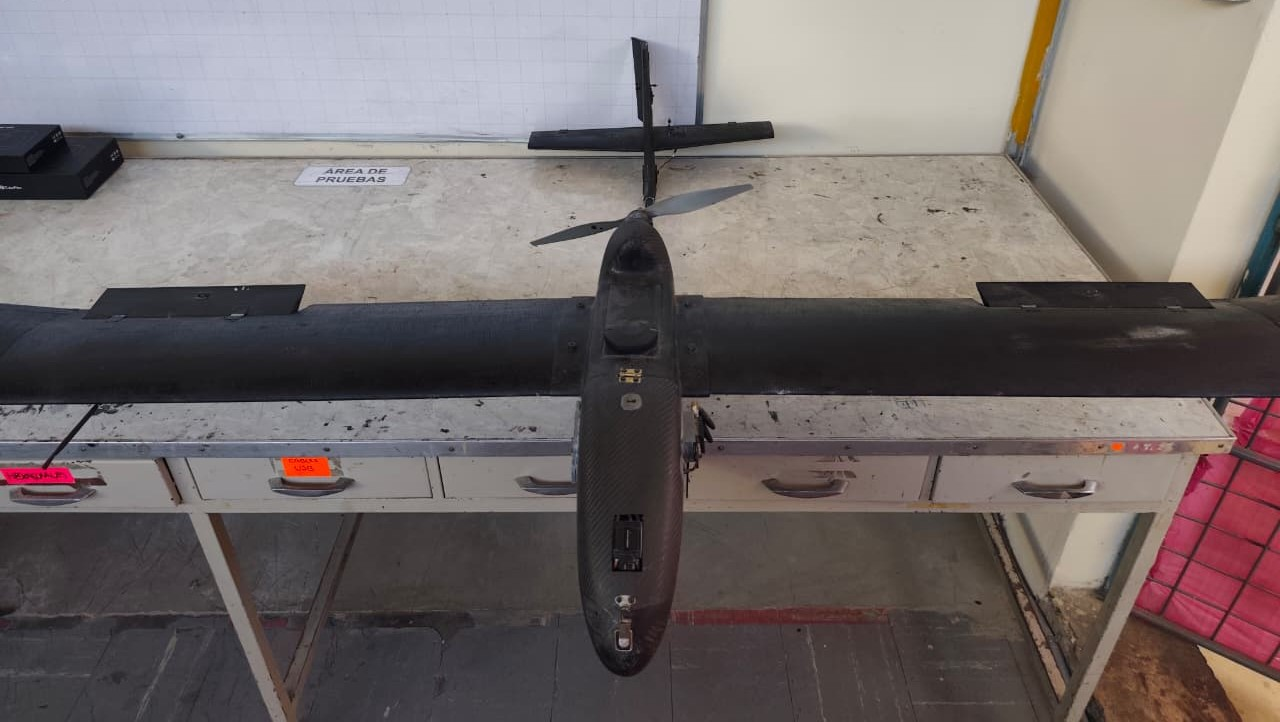
\includegraphics[width=0.9\textwidth]{Fix_wing.jpeg}
    \caption{Vista general de la plataforma de ala fija. Destaca su fuselaje de fibra de carbono, alas rectas, empenaje convencional y configuración de propulsión tipo \textit{pusher} (motor trasero).}
    \label{fig:plataforma_alafija}
\end{figure}

\subsection{Arquitectura del Sistema de Control}
A diferencia de los cuadricópteros, el ala fija basa su sustentación en la aerodinámica generada por el flujo de aire sobre sus perfiles alares. El controlador de vuelo ejecuta cientos de correcciones por segundo para mantener la estabilidad en los ejes de alabeo (roll), cabeceo (pitch) y guiñada (yaw) utilizando superficies de control (alerones, elevador, timón).

\section{Lista de Componentes del Sistema}
Esta sección detalla los componentes electrónicos instalados en el fuselaje de fibra de carbono:
\begin{itemize}
    \item \textbf{Controlador de Vuelo (FC):} \textbf{Cube Orange} con Carrier Board, proporcionando IMUs redundantes y conectividad JST-GH.
    \item \textbf{Gestión de Potencia:} Sistema \textbf{Mauch} (PL-Sensor y BEC) para medición de grado industrial de corriente/voltaje y alimentación limpia a 5.3V.
    \item \textbf{Sistema de Propulsión:} \textbf{ESC Hobbywing} expuesto al flujo de aire para refrigeración pasiva, y motor brushless.
    \item \textbf{Receptor de Radio:} \textbf{FrSky X8R} de 8/16 canales, conectado vía protocolo SBUS y transmitiendo telemetría por \textit{Smart Port}.
    \item \textbf{Expansión I2C:} \textbf{Hub/Splitter} montado en el chasis para la conexión simultánea de periféricos I2C como el magnetómetro externo y el tubo de Pitot.
\end{itemize}

\section{Configuración del Hardware y Enlaces}

\subsection{Diferenciación de Enlaces (Telemetría vs. Control)}
El sistema requiere dos enlaces de comunicación paralelos: el enlace de control directo a 2.4 GHz (Radio FrSky X8R) para baja latencia, y el enlace de telemetría bidireccional (generalmente a 915 MHz con módulos RFD900) conectado al puerto TELEM 1 del Cube Orange para el monitoreo de la misión en Mission Planner.

\subsection{Conexiones Centrales del Controlador Cube}
\begin{itemize}
    \item \textbf{RC IN:} Conectado a la salida SBUS del FrSky X8R.
    \item \textbf{POWER 1:} Conectado al BEC de la placa Mauch.
    \item \textbf{MAIN OUT:} Mapeo de las señales PWM hacia los servos (ej. CH1: Alerones, CH2: Elevador, CH3: Acelerador/ESC Hobbywing, CH4: Timón).
\end{itemize}

\section{Sincronización de ESC y Configuración de Arranque}
Para garantizar que el motor responda correctamente a todo el rango del acelerador:
\begin{enumerate}
    \item Retirar la hélice del motor por seguridad.
    \item Encender la emisora FrSky y subir el acelerador al 100\%.
    \item Conectar la batería principal al sistema (a través del PL-Sensor de Mauch).
    \item El ESC \textbf{Hobbywing} emitirá tonos musicales. Inmediatamente, bajar el acelerador al 0\%.
    \item Esperar el tono de confirmación del ESC, indicando que los límites PWM han sido memorizados.
\end{enumerate}

\section{Calibraciones Específicas de Ala Fija (ArduPlane)}

\subsection{Calibración del Tubo de Pitot (Airspeed)}
En alas fijas, conocer la velocidad relativa al aire es crucial para evitar la pérdida (stall). El sensor conectado al Hub I2C debe calibrarse antes de cada vuelo. En Mission Planner, se debe ejecutar la \textit{Preflight Calibration} asegurándose de que la sonda de Pitot esté completamente cubierta para establecer la presión cero.

\subsection{Compensación de Altitud en Ecosistemas Altoandinos}
Operar en ubicaciones de elevada altitud topográfica (como Quito, a $\sim$2800 m.s.n.m.) impacta el rendimiento aerodinámico debido a la menor densidad del aire. 
\begin{itemize}
    \item \textbf{Velocidad de Pérdida (Stall Speed):} La velocidad respecto al suelo (\textit{True Airspeed}) será mayor.
    \item \textbf{Ajuste de Parámetros:} Se deben revisar los parámetros \texttt{TRIM\_ARSPD\_CM} (velocidad de crucero) y \texttt{ARSPD\_FBW\_MIN} (velocidad mínima estabilizada) en Mission Planner para asegurar un margen seguro sobre la velocidad de pérdida real en estas condiciones.
\end{itemize}

\end{document}
